\documentclass[letterpaper,twocolumn, 11pt]{article}

\usepackage{graphicx}
\usepackage[top=1in, bottom=1in, left=1in, right=1in]{geometry}
\usepackage[dvips]{hyperref}
\usepackage{amsmath}

\author{Luke Fraser}
\title{Programming Assignment 2: \\ Mandelbrot Set Fractal}
\date{02/05/15}

\begin{document}
\maketitle
\begin{abstract}
In this project we were tasked with implementing a GPU and CPU based Mandelbrot set generator. The images generated by the Mandelbrot set form a fractal that looks quite interesting.
\end{abstract}

\section{Introduction}
The Mandelbrot set is calculated form a set of simple equations as seen in equations below.
\begin{equation}
  M={c \in C| \lim_{n \to \infty}Z_n \neq \infty}
\end{equation}
\begin{equation}
  z_0=c
\end{equation}
\begin{equation}
  Z_{n+1}=Z_n^2+c
\end{equation}

These equations were used to generate the Mandelbrot fractal images. However many times you recurse with the equation is the number of iterations of the Mandelbrot you take. In the case of this assignment 1024 iterations were used to increase the running time of the algorithm. Each pixel in the image will be run a maximum of 1024 times. This is an important distinction as each of the pixel will not run this many iterations of itself. A pixel is considered not a part of the Mandelbrot set if after the max iterations is found to be smaller than 2. This is because it is known that after a number in the set goes beyond 2 it will not loop back below 2 again.

\begin{figure}
  \centering
  
\includegraphics[width=7cm]{mandelbrot.png}
  \caption{2000x2000 pixel Mandelbrot image generated from GPU: 1024 iterations.}
  \label{fig:mandelbrot}
\end{figure}
All pixels that are considered apart of the set will run the maximum number of iterations, but the pixels that are black will only run the number of iterations that it takes to go beyond 2. This is an important run-time consideration to make. As the numbers used to build the Mandelbrot as well as the zoom level of the set will have a significant impact the running time of the image. If every pixel of the image were a part of the Mandelbrot set them every pixel would need to run 1024 times and this would slow the production down. As well in reverse the more pixels that diverge quickly to Infinity require less processing time an can be discarded quickly. This means the more black pixels in the image the fast the image can be generated. Assuming there is a single white pixel in the image the algorithm would take at least as long as it takes to iterate the algorithm 1024 times. This is assuming each pixel can be performed in parallel simultaneously.

\section{Implementation}
The implementation of the CPU code was based on the online tutorial presented in the project description. As well the GPU code was also heavily based on the tutorial code.

The GPU code operated with threads being dispersed over rows of the image and the program was passed the desired blocks per row and the blocks and threads were calculated from that number. This allowed the memory to be accessed in a sequential manner as each block would access a particular chuck of a given row of the image. As well each image array was stored in single 1d array. In the function I developed two arrays were used to record the necessary information to generate the Mandelbrot image. I recorded the standard black and white values of the image, but I also recorded the number of iterations below 1024 a particular pixel took to go beyond 2. The second array was important for coloring the image later.
\subsection{Results}
\begin{figure}
  \centering
  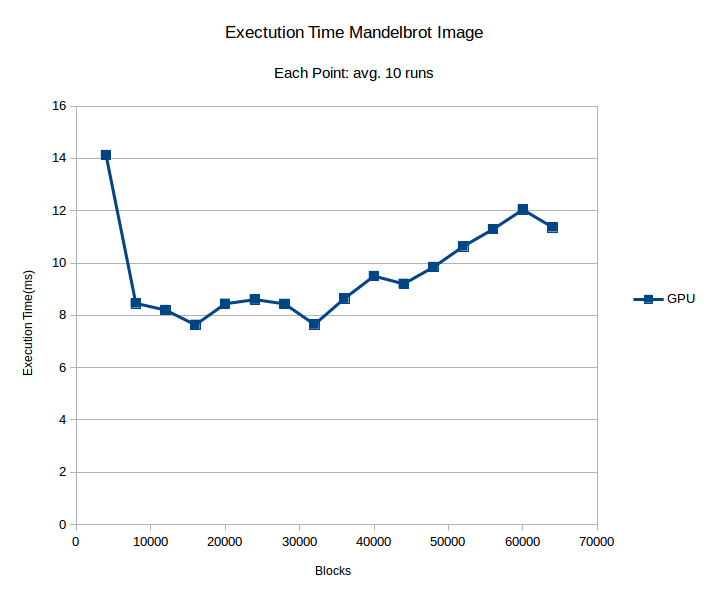
\includegraphics[width=7.5cm]{graph.png}
  \caption{Graph of execution time of the Mandelbrot image. Each point is the average of 10 runs.}
  \label{fig:graph}
\end{figure}

The results of the GPU program are shown in figure~\ref{fig:graph}. The GPU code performed a maximum speed-up of 795.73\%. This is a huge performance improvement over the sequential CPU based method. The computer on average ran created the image in 6074.41 milliseconds.

It was an incredibly slow process for the CPU to generate the image compared to the GPU.


\end{document}

